% !TeX program = xelatex
\documentclass[a4paper,10pt]{article}

% ============================================================================
% កញ្ចប់បណ្ណាល័យ (Packages) – តាមលំនាំ NGS Preah Krasang (ls_plan.tex)
% បរិបទ៖ គ្មានស្លាយ LCD និងគ្មានម៉ាស៊ីនគិតលេខ — ប្រើសន្លឹកកិច្ចការសិស្ស (ស-ខ្មៅ) និងក្ដារខៀនជាគោល
% ============================================================================
\usepackage[a4paper, left=0.95cm, right=0.95cm, top=0.85cm, bottom=0.92cm, footskip=0.52cm]{geometry}
\usepackage{amsmath}
\usepackage{unicode-math}
\usepackage{fontspec}
\usepackage{array, longtable, multirow, colortbl}
\usepackage[table]{xcolor}
\usepackage{enumitem}
\usepackage{pifont}
\usepackage{fancyhdr}
\usepackage{tikz}
\usetikzlibrary{calc, arrows.meta, angles, quotes, decorations.markings, decorations.pathreplacing, patterns, babel}

\makeatletter
\let\@expl@@@mark@update@singlecol@structures@@\relax
\makeatother

\providecommand{\NGSFindFonts}{%
  \IfFileExists{C:/Windows/Fonts/cambria.ttc}{%
    \def\NGSSysPath{C:/Windows/Fonts/}%
    \def\NGSUserPath{C:/Users/KIT/AppData/Local/Microsoft/Windows/Fonts/}%
  }{%
    \IfFileExists{./fonts/KhmerOSsiemreap.ttf}{\def\NGSSysPath{./fonts/}\def\NGSUserPath{./fonts/}}{%
    \IfFileExists{../fonts/KhmerOSsiemreap.ttf}{\def\NGSSysPath{../fonts/}\def\NGSUserPath{../fonts/}}{%
    \IfFileExists{../../fonts/KhmerOSsiemreap.ttf}{\def\NGSSysPath{../../fonts/}\def\NGSUserPath{../../fonts/}}{%
    \IfFileExists{../../../fonts/KhmerOSsiemreap.ttf}{\def\NGSSysPath{../../../fonts/}\def\NGSUserPath{../../../fonts/}}{%
    \IfFileExists{../../../../fonts/KhmerOSsiemreap.ttf}{\def\NGSSysPath{../../../../fonts/}\def\NGSUserPath{../../../../fonts/}}{%
    \IfFileExists{../../../../../fonts/KhmerOSsiemreap.ttf}{\def\NGSSysPath{../../../../../fonts/}\def\NGSUserPath{../../../../../fonts/}}{%
    \IfFileExists{../../../../../../fonts/KhmerOSsiemreap.ttf}{\def\NGSSysPath{../../../../../../fonts/}\def\NGSUserPath{../../../../../../fonts/}}{%
      \def\NGSSysPath{../../../../../../../fonts/}\def\NGSUserPath{../../../../../../../fonts/}%
    }}}}}}}%
  }%
}
\NGSFindFonts

\setmathfont[Path={\NGSSysPath}, FontIndex=1, Scale=1.02]{cambria.ttc}
\defaultfontfeatures{Ligatures=TeX}

\setmainfont[
  Path={\NGSUserPath}, Extension=.ttf, Script=Khmer,
  BoldFont={KhmerOSsiemreap}, BoldFeatures={FakeBold=1.8},
  ItalicFont={KhmerOSsiemreap}, ItalicFeatures={FakeSlant=0.25},
  BoldItalicFont={KhmerOSsiemreap}, BoldItalicFeatures={FakeBold=1.8, FakeSlant=0.25}
]{KhmerOSsiemreap}

\newfontfamily\muol[Path={\NGSUserPath}, Extension=.ttf, Script=Khmer]{KhmerOSmuollight}
\newfontfamily\TimesEn[Path={\NGSSysPath}, Extension=.ttf, Scale=1.00, BoldFont={timesbd}, ItalicFont={timesi}, BoldItalicFont={timesbi}]{times}
\newfontfamily\NagaBold[Path={\NGSUserPath}, Extension=.ttf]{AKbalthom Naga Bold}
\newfontfamily\CalibriFont[Path={\NGSSysPath}, Extension=.ttf]{calibri}
\newfontfamily\Tacteing[Path={\NGSUserPath}]{TACTENG.TTF}
\newfontfamily\CourierBullet[Path={\NGSSysPath}, Extension=.ttf]{cour}
\newcommand{\wcirc}{{\CourierBullet\fontsize{9.5pt}{11pt}\selectfont o}}

\XeTeXlinebreaklocale "km"
\XeTeXlinebreakskip = 0pt plus 1pt minus 0.1pt

\definecolor{stepgray}{HTML}{D9D9D9}
\definecolor{headgray}{HTML}{F2F2F2}
\definecolor{boxgray}{HTML}{D9D9D9}
\definecolor{darkred}{HTML}{C00000}
\definecolor{red5e}{HTML}{FF0000}

\pagestyle{fancy}
\fancyhf{}
\renewcommand{\headrulewidth}{0pt}
\fancyfoot[R]{\CalibriFont\fontsize{11pt}{13pt}\selectfont\thepage}

\setlength{\parindent}{0pt}
\setlength{\parskip}{0pt}
\setlength{\tabcolsep}{3.8pt}

\newcolumntype{L}[1]{>{\raggedright\arraybackslash}p{#1}}
\newcolumntype{C}[1]{>{\centering\arraybackslash}p{#1}}

\newcommand{\en}[1]{{\TimesEn #1}}
\newcommand{\enbf}[1]{{\TimesEn\textbf{#1}}}
\newcommand{\unit}[1]{\,\text{\en{#1}}}
\newcommand{\fiveE}[1]{{\NagaBold\fontsize{9.5pt}{13pt}\selectfont\textcolor{red5e}{#1}}}
\newcommand{\timenote}[1]{\textcolor{darkred}{\textit{#1}}}
\newcommand{\redsub}[1]{\textcolor{darkred}{#1}}
\newcommand{\graybox}[1]{\colorbox{boxgray}{\strut\hspace{2pt}#1\hspace{2pt}}}
\newcommand{\ditem}{\tikz[baseline=-0.5ex]\fill (0,0.42ex) -- (0.42ex,0) -- (0,-0.42ex) -- (-0.42ex,0) -- cycle;\hspace{0.3em}}
\newcommand{\cnum}[1]{{\fontsize{10.5pt}{12pt}\selectfont\ding{\numexpr181+#1\relax}}\hspace{0.15em}}
\newcommand{\cfig}[1]{\par\vspace{3pt}{\centering #1\par}\vspace{3pt}}
\newcommand{\stepheader}[1]{\multicolumn{3}{|c|}{\cellcolor{stepgray}\muol #1} \\* \noalign{\hrule height 0.4pt}}
\newcommand{\khmflourish}{{\Tacteing\fontsize{36pt}{14pt}\selectfont\raisebox{-5pt}{3}}}

% ============================================================================
% ម៉ាក្រូគូសរូប TikZ ស-ខ្មៅ ១០០% សម្រាប់មេរៀន ៣.២.៦ ការប្រាក់សមាស (CINT)
% ============================================================================

% ១. E1 Engage: មីងសៅដាក់ប្រាក់សមាស ទល់នឹង ការប្រាក់សាមញ្ញ (ទំ.៣៧)
\newcommand{\figEngageCINT}{%
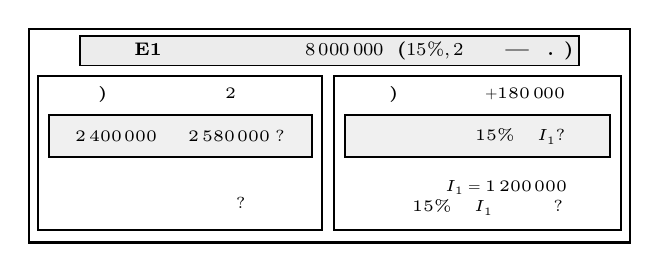
\begin{tikzpicture}[x=0.96cm, y=0.92cm, every node/.style={font=\scriptsize, text=black}]
  \draw[black, line width=0.95pt] (0,0) rectangle (7.95,2.95);
  \node[fill=gray!15, draw=black, line width=0.6pt, inner sep=2pt, font=\fontsize{6.6pt}{8.4pt}\selectfont\bfseries] at (3.975,2.65) {បេសកកម្ម \en{E1}៖ ប្រាក់បញ្ញើសមាសរបស់មីងសៅ $8\,000\,000\text{៛}$ ($15\%, 2$ ឆ្នាំ — ទំ.៣៧)};

  \draw[black, line width=0.8pt] (0.12,0.18) rectangle (3.88,2.30);
  \node[font=\fontsize{5.8pt}{7.5pt}\selectfont\bfseries] at (2.00,2.04) {១) ការប្រាក់សមាសសរុបរយៈពេល $2$ ឆ្នាំ};
  \draw[black, line width=0.75pt, fill=gray!12] (0.26,1.18) rectangle (3.74,1.76);
  \node[font=\fontsize{5.8pt}{7.5pt}\selectfont] at (2.00,1.47) {$2\,400\,000\text{៛}$ \;ឬ\; $2\,580\,000\text{៛}$?};
  \node[align=center, font=\fontsize{5.8pt}{7.4pt}\selectfont] at (2.00,0.62) {តើស្មើការប្រាក់សាមញ្ញដែរឬទេ\\ពេលបូកការប្រាក់ចូលប្រាក់ដើម?};

  \draw[black, line width=0.8pt] (4.04,0.18) rectangle (7.83,2.30);
  \node[font=\fontsize{5.8pt}{7.5pt}\selectfont\bfseries] at (5.935,2.04) {២) ប្រភពនៃប្រាក់លើស $+180\,000\text{៛}$};
  \draw[black, line width=0.75pt, fill=gray!12] (4.18,1.18) rectangle (7.69,1.76);
  \node[font=\fontsize{5.8pt}{7.5pt}\selectfont] at (5.935,1.47) {ប្រាក់រង្វាន់ \;ឬ\; $15\%$ លើ $I_1$?};
  \node[align=center, font=\fontsize{5.8pt}{7.4pt}\selectfont] at (5.935,0.62) {ឆ្នាំទី១ បាន $I_1 = 1\,200\,000\text{៛}$\\ចុះ $15\%$ នៃ $I_1$ ស្មើប៉ុន្មាន?};
\end{tikzpicture}}

% ២. E2 POE 2: ខ្សែសង្វាក់បង្វិលប្រាក់ដើម ៣ ឆ្នាំរបស់ទ្រាចាន់ (គំរូ ១ ទំ.៣៧-៣៨)
\newcommand{\figRolloverCINT}{%
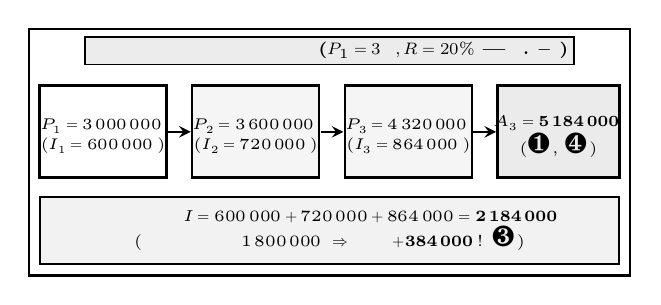
\begin{tikzpicture}[x=0.96cm, y=0.92cm, every node/.style={font=\scriptsize, text=black}]
  \draw[black, line width=0.95pt] (0,0) rectangle (7.95,3.40);
  \node[fill=gray!15, draw=black, line width=0.6pt, inner sep=2pt, font=\fontsize{6.0pt}{7.8pt}\selectfont\bfseries] at (3.975,3.10) {ខ្សែសង្វាក់បង្វិលប្រាក់ដើម ៣ ឆ្នាំរបស់ទ្រាចាន់ ($P_1=3\text{លាន}, R=20\%$ — ទំ.៣៧–៣៨)};

  % 4 stage boxes
  \draw[black, line width=0.8pt] (0.14,1.35) rectangle (1.82,2.62);
  \node[align=center, font=\fontsize{5.6pt}{7.2pt}\selectfont] at (0.98,1.98) {\textbf{ដើមឆ្នាំទី១}\\$P_1 = 3\,000\,000\text{៛}$\\($I_1 = 600\,000\text{៛}$)};

  \draw[->, >=stealth, line width=0.85pt] (1.84,1.98) -- (2.14,1.98);

  \draw[black, line width=0.8pt, fill=gray!8] (2.16,1.35) rectangle (3.84,2.62);
  \node[align=center, font=\fontsize{5.6pt}{7.2pt}\selectfont] at (3.00,1.98) {\textbf{ដើមឆ្នាំទី២}\\$P_2 = 3\,600\,000\text{៛}$\\($I_2 = 720\,000\text{៛}$)};

  \draw[->, >=stealth, line width=0.85pt] (3.86,1.98) -- (4.16,1.98);

  \draw[black, line width=0.8pt, fill=gray!8] (4.18,1.35) rectangle (5.86,2.62);
  \node[align=center, font=\fontsize{5.6pt}{7.2pt}\selectfont] at (5.02,1.98) {\textbf{ដើមឆ្នាំទី៣}\\$P_3 = 4\,320\,000\text{៛}$\\($I_3 = 864\,000\text{៛}$)};

  \draw[->, >=stealth, line width=0.85pt] (5.88,1.98) -- (6.18,1.98);

  \draw[black, line width=0.9pt, fill=gray!16] (6.20,1.35) rectangle (7.81,2.62);
  \node[align=center, font=\fontsize{5.6pt}{7.2pt}\selectfont] at (7.005,1.98) {\textbf{ចុងឆ្នាំទី៣}\\$A_3 = \mathbf{5\,184\,000\text{៛}}$\\(\cnum{1}, \cnum{4})};

  % Summary bar
  \draw[black, line width=0.75pt, fill=gray!10] (0.14,0.16) rectangle (7.81,1.08);
  \node[align=center, font=\fontsize{5.7pt}{7.3pt}\selectfont] at (3.975,0.62) {\textbf{ការប្រាក់សមាសសរុប៖} $I = 600\,000 + 720\,000 + 864\,000 = \mathbf{2\,184\,000\text{៛}}$\\(ធៀបនឹងការប្រាក់សាមញ្ញ $1\,800\,000\text{៛}$ $\Rightarrow$ សមាសលើស $+\mathbf{384\,000\text{៛}}$! \cnum{3})};
\end{tikzpicture}}

% ៣. E4 Worked Example: គំរូទី២ គិតការប្រាក់សមាសរាល់កន្លះឆ្នាំម្ដង (ទំ.៣៨)
\newcommand{\figSemiAnnualCINT}{%
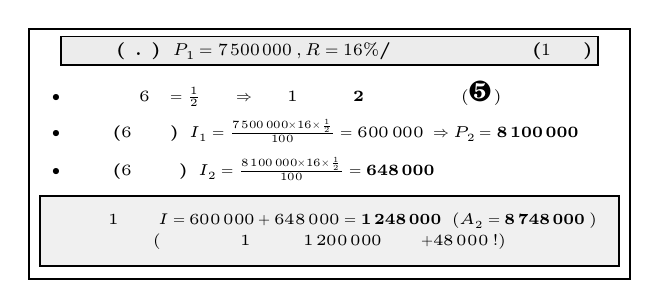
\begin{tikzpicture}[x=0.96cm, y=0.92cm, every node/.style={font=\scriptsize, text=black}]
  \draw[black, line width=0.95pt] (0,0) rectangle (7.95,3.45);
  \node[fill=gray!15, draw=black, line width=0.6pt, inner sep=2pt, font=\fontsize{6.2pt}{8.0pt}\selectfont\bfseries] at (3.975,3.15) {គំរូទី ២ (ទំ.៣៨)៖ $P_1 = 7\,500\,000\text{៛}, R = 16\%$/ឆ្នាំ គិតសមាសរាល់កន្លះឆ្នាំ ($1$ ឆ្នាំ)};

  \node[anchor=west, font=\fontsize{5.7pt}{7.4pt}\selectfont] at (0.18,2.56) {$\bullet$ \textbf{ច្រកកន្លះឆ្នាំ៖} $6\text{ ខែ} = \frac{1}{2}\text{ ឆ្នាំ}$ $\Rightarrow$ ក្នុង $1$ ឆ្នាំ មាន $\mathbf{2}$ \textbf{គ្រាបង្វិលប្រាក់ដើម} (\cnum{5})};
  \node[anchor=west, font=\fontsize{5.7pt}{7.4pt}\selectfont] at (0.18,2.04) {$\bullet$ \textbf{គ្រាទី ១ ($6$ ខែដំបូង)៖} $I_1 = \frac{7\,500\,000\times 16\times \frac{1}{2}}{100} = 600\,000\text{៛} \Rightarrow P_2 = \mathbf{8\,100\,000\text{៛}}$};
  \node[anchor=west, font=\fontsize{5.7pt}{7.4pt}\selectfont] at (0.18,1.52) {$\bullet$ \textbf{គ្រាទី ២ ($6$ ខែបន្ទាប់)៖} $I_2 = \frac{8\,100\,000\times 16\times \frac{1}{2}}{100} = \mathbf{648\,000\text{៛}}$};

  \draw[black, line width=0.75pt, fill=gray!12] (0.14,0.18) rectangle (7.81,1.14);
  \node[align=center, font=\fontsize{5.6pt}{7.3pt}\selectfont] at (3.975,0.66) {\textbf{សរុបក្នុង $1$ ឆ្នាំ៖} $I = 600\,000 + 648\,000 = \mathbf{1\,248\,000\text{៛}}$ ($A_2 = \mathbf{8\,748\,000\text{៛}}$)\\(ធំជាងការប្រាក់គិត $1$ ឆ្នាំម្ដង $1\,200\,000\text{៛}$ ចំនួន $+48\,000\text{៛}$!)};
\end{tikzpicture}}

% ៤. E5 Diagnostic Options A-D
\newcommand{\figExitCardsCINT}{%
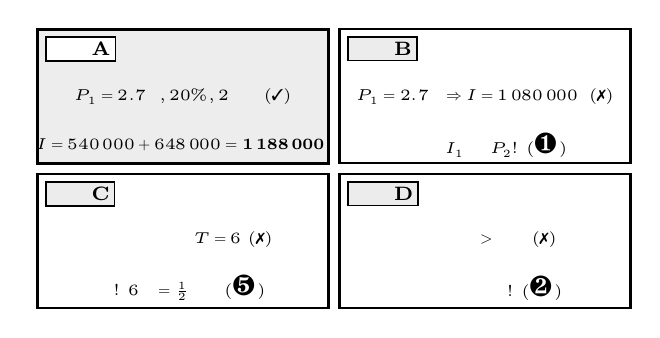
\begin{tikzpicture}[x=0.96cm, y=0.92cm, every node/.style={font=\scriptsize, text=black}]
  \draw[black, line width=1.1pt, fill=gray!14] (0,2.00) rectangle (3.85,3.85);
  \node[anchor=north west, fill=white, draw=black, line width=0.6pt, inner sep=1.8pt] at (0.10,3.75) {\textbf{ជម្រើស \en{A}}};
  \node[font=\fontsize{5.7pt}{7.4pt}\selectfont] at (1.925,2.92) {$P_1=2.7\text{លាន}, 20\%, 2$ ឆ្នាំ (\ding{51})};
  \node[font=\fontsize{5.7pt}{7.4pt}\selectfont] at (1.925,2.25) {$I = 540\,000 + 648\,000 = \mathbf{1\,188\,000\text{៛}}$};

  \draw[black, line width=0.9pt] (4.00,2.00) rectangle (7.85,3.85);
  \node[anchor=north west, fill=gray!15, draw=black, line width=0.6pt, inner sep=1.8pt] at (4.10,3.75) {\textbf{ជម្រើស \en{B}}};
  \node[font=\fontsize{5.7pt}{7.4pt}\selectfont] at (5.925,2.92) {$P_1=2.7\text{លាន} \Rightarrow I = 1\,080\,000\text{៛}$ (\ding{55})};
  \node[font=\fontsize{5.7pt}{7.4pt}\selectfont] at (5.925,2.25) {ភ្លេចបូក $I_1$ ចូល $P_2$! (\cnum{1})};

  \draw[black, line width=0.9pt] (0,0) rectangle (3.85,1.85);
  \node[anchor=north west, fill=gray!15, draw=black, line width=0.6pt, inner sep=1.8pt] at (0.10,1.75) {\textbf{ជម្រើស \en{C}}};
  \node[font=\fontsize{5.7pt}{7.4pt}\selectfont] at (1.925,0.95) {កន្លះឆ្នាំម្ដង៖ ជំនួស $T=6$ (\ding{55})};
  \node[font=\fontsize{5.7pt}{7.4pt}\selectfont] at (1.925,0.28) {ខុស! $6\text{ ខែ} = \frac{1}{2}\text{ ឆ្នាំ}$ (\cnum{5})};

  \draw[black, line width=0.9pt] (4.00,0) rectangle (7.85,1.85);
  \node[anchor=north west, fill=gray!15, draw=black, line width=0.6pt, inner sep=1.8pt] at (4.10,1.75) {\textbf{ជម្រើស \en{D}}};
  \node[font=\fontsize{5.7pt}{7.4pt}\selectfont] at (5.925,0.95) {ឆ្នាំទី១ សមាស $>$ សាមញ្ញ (\ding{55})};
  \node[font=\fontsize{5.7pt}{7.4pt}\selectfont] at (5.925,0.28) {គ្រាទី១ គឺស្មើគ្នាដដែល! (\cnum{2})};
\end{tikzpicture}}

\begin{document}
\fontsize{10pt}{15.2pt}\selectfont

% -------------------- ក្បាលកិច្ចតែងការ --------------------
\begin{center}
  {\muol\fontsize{11pt}{16pt}\selectfont ព្រះរាជាណាចក្រកម្ពុជា}\\[2pt]
  {\muol\fontsize{10pt}{15pt}\selectfont ជាតិ សាសនា ព្រះមហាក្សត្រ}\\[1pt]
  \khmflourish
\end{center}

\vspace{-24pt}
{\muol\fontsize{9.5pt}{12.5pt}\selectfont
មន្ទីរអប់រំ យុវជន និងកីឡា ខេត្តកំពង់ធំ\\
ការិយាល័យអប់រំ យុវជន និងកីឡា ស្រុកកំពង់ស្វាយ\\
អនុវិទ្យាល័យព្រះក្រសាំង}

\vspace{1pt}
\begin{center}
  {\muol\fontsize{10pt}{14pt}\selectfont កិច្ចតែងការបង្រៀន}
\end{center}
\vspace{0pt}

% -------------------- ព័ត៌មានទូទៅ --------------------
{\renewcommand{\arraystretch}{0.98}
\hspace*{3.1cm}%
\begin{tabular}{@{}l l L{11.0cm}@{}}
  - \hspace{0.35cm} មុខវិជ្ជា & : & គណិតវិទ្យា ថ្នាក់ទី៨ (ពីជគណិត) \\
  - \hspace{0.35cm} ចំណងជើងមេរៀន & : & មេរៀនទី៣៖ ទំហំសមាមាត្រ និងភាគរយ \\
  - \hspace{0.35cm} ចំណងជើងរង & : & ២.៦. ការប្រាក់សមាស (ទំ.៣៧–៣៨ និងលំហាត់ \#17, \#18 ទំ.៤២) \\
  - \hspace{0.35cm} រយៈពេល & : & ១ ម៉ោងសិក្សា (៥០ នាទី) \\
  - \hspace{0.35cm} បង្រៀនដោយ & : & ហុក ប៊ុនថែន \\
  - \hspace{0.35cm} កាលបរិច្ឆេទ & : & ថ្ងៃពុធ ទី២ ខែធ្នូ ឆ្នាំ២០២៦ \\
\end{tabular}

\vspace{2pt}

% -------------------- I. វត្ថុបំណង --------------------
\textbf{I.} {\muol វត្ថុបំណង}\\[1pt]
\hspace*{0.55cm}%
\begin{tabular}{@{}l l L{14.2cm}@{}}
  \wcirc \hspace{0.25cm} វិជ្ជាសម្បទា & : & សិស្សប្រាប់និយមន័យនៃការប្រាក់សមាស និងលក្ខណៈខុសគ្នារវាងការប្រាក់សមាស ($P_{k+1} = P_k + I_k$) ធៀបនឹងការប្រាក់សាមញ្ញបានត្រឹមត្រូវ ។ \\
  \wcirc \hspace{0.25cm} បំណិនសម្បទា & : & សិស្សគណនាការប្រាក់សមាស និងប្រាក់សរុបតាមតារាងបង្វិលប្រាក់ដើមប្រចាំឆ្នាំ និងរាល់កន្លះឆ្នាំម្ដង ($T = \frac{1}{2}$ ឆ្នាំ, ទំ.៣៧–៣៨) ដោយដៃលើសន្លឹកកិច្ចការ ។ \\
  \wcirc \hspace{0.25cm} ចរិយាសម្បទា & : & សិស្សយល់ដឹងពីអានុភាពនៃការប្រាក់សមាសក្នុងការសន្សំប្រាក់រយៈពេលវែង និងប្រុងប្រយ័ត្នចំពោះបំណុលការប្រាក់សមាសក្នុងជីវភាពរស់នៅ ។ \\
\end{tabular}

\vspace{2pt}

% -------------------- II. សម្ភារៈឧបទេស --------------------
\textbf{II.} {\muol សម្ភារៈឧបទេស}\\[1pt]
\hspace*{0.55cm}$\bullet$ \hspace{0.35cm} សៀវភៅសិក្សាគោលគណិតវិទ្យាថ្នាក់ទី៨ (ទំ.៣៧–៣៨, ៤២) ក្ដារខៀន ដីស និងសន្លឹកកិច្ចការសិស្ស ស-ខ្មៅ (\en{Worksheet\_CINT} ទំព័រ ១–២ គ្មានស្លាយ \en{LCD})

\vspace{2pt}

% -------------------- III. វិធីសាស្រ្តបង្រៀន --------------------
\textbf{III.} {\muol វិធីសាស្រ្តបង្រៀន}\\[1pt]
\hspace*{0.45cm}%
\begin{tabular}{@{}l l L{14.85cm}@{}}
  $\bullet$ \hspace{0.25cm} គោលវិធី & : & សិស្សមជ្ឈមណ្ឌល (បង្រៀនតាមសន្លឹកកិច្ចការស៊ើបអង្កេត និងក្ដារខៀន គ្មាន \en{LCD}) \\
  $\bullet$ \hspace{0.25cm} យុទ្ធវិធីបង្រៀន & : & គំរូ \en{5Es} រួមបញ្ចូលតារាងបញ្ជីបង្វិលប្រាក់ដើមតាមគ្រា (\en{Period-by-Period Rollover Ledger}) \\
\end{tabular}
}

\vspace{2pt}

% -------------------- IV. ដំណើរការបង្រៀន --------------------
\textbf{IV.} {\muol ដំណើរការបង្រៀន}

\vspace{1pt}

\renewcommand{\arraystretch}{1.15}
\begin{longtable}{|L{5.50cm}|L{7.90cm}|L{4.80cm}|}
\hline
\rowcolor{headgray}
\multicolumn{1}{|c|}{\muol សកម្មភាពគ្រូ} &
\multicolumn{1}{c|}{\muol ខ្លឹមសារមេរៀន} &
\multicolumn{1}{c|}{\muol សកម្មភាពសិស្ស} \\
\hline
\endfirsthead
\hline
\endhead
\hline
\endfoot
\hline
\endlastfoot

% ==================== ជំហានទី១ (2min) ====================
\stepheader{ជំហានទី១ \enbf{(}រដ្ឋបាលថ្នាក់\enbf{)}}
$\bullet$ ពិនិត្យអវត្តមាន អនាម័យ និងសណ្ដាប់ធ្នាប់ថ្នាក់រៀន
&
$\bullet$ រដ្ឋបាលថ្នាក់ និងការរៀបចំដៃគូសិក្សា
&
$\circ$ ប្រធានថ្នាក់រាយការណ៍អវត្តមាន \\[3pt]

$\bullet$ ចែក \textbf{សន្លឹកកិច្ចការសិស្ស (\en{Worksheet\_CINT})} ម្នាក់ ១ សន្លឹក (ផ្កាប់ទុកសិន)
&
$\bullet$ សន្លឹកកិច្ចការសិស្ស ស-ខ្មៅ (\en{Worksheet\_CINT} ទំព័រ ១–២)
&
$\circ$ ទទួលសន្លឹកកិច្ចការ និងត្រៀមសម្ភារៈសរសេរ \\
\hline

% ==================== ជំហានទី២ (9min: <=3 + 3 + E1 3) ====================
\stepheader{ជំហានទី២ \enbf{(}កិច្ចការផ្ទះ \enbf{+} ទំនាក់ទំនងមេរៀនថ្មី\enbf{)}}
\ditem \textbf{កំណែកិច្ចការផ្ទះ ($\le 3\unit{min}$)} \timenote{(កុំសរសេរវែង)} \par
$\bullet$ ហៅសិស្ស ២ នាក់ឡើងសរសេរចម្លើយលំហាត់ \#16 ក, ខ, គ (ទំ.៤២) លើក្ដារខៀន
&
{\centering\redsub{កំណែកិច្ចការផ្ទះមេរៀន ២.៥ (ទំ.៤២ \#16 ក, ខ, គ)}\par} \par
$\bullet$ \textbf{\#16 ក-ខ៖} គណនាការប្រាក់សាមញ្ញតាម $I = \frac{PRT}{100}$ និងប្រាក់សរុប $A = P+I$ \par
$\bullet$ \textbf{\#16 គ៖} ប្ដូររយៈពេលខែជាប្រភាគនៃឆ្នាំ ($T = \frac{m}{12}$) មុនជំនួសលេខ
&
$\circ$ ផ្ទៀងផ្ទាត់ និងកែតម្រូវចម្លើយក្នុងសៀវភៅកិច្ចការផ្ទះ \\[3pt]

\ditem \textbf{រំលឹកមេរៀនទាក់ទង (3min)} \par
$\bullet$ សួររហ័ស៖ បើដាក់ប្រាក់ $8\,000\,000\text{៛}$ អត្រា $15\%$/ឆ្នាំ តើការប្រាក់ក្នុង $1$ ឆ្នាំស្មើប៉ុន្មាន?
&
{\centering\redsub{រំលឹកការប្រាក់ក្នុង ១ ឆ្នាំ និងកន្លះឆ្នាំ}\par} \par
$\bullet$ ក្នុង $1$ ឆ្នាំ៖ $I_1 = \frac{8\,000\,000 \times 15 \times 1}{100} = \mathbf{1\,200\,000\text{៛}}$
&
$\circ$ គណនារហ័សថាស្មើ $1\,200\,000\text{៛}$ \\[3pt]

$\bullet$ សួររហ័សបន្ត៖ ចុះបើគិតការប្រាក់ក្នុងរយៈពេលកន្លះឆ្នាំ ($6$ ខែ) រយៈពេល $T$ ស្មើប៉ុន្មានឆ្នាំ?
&
$\bullet$ កន្លះឆ្នាំ ($6$ ខែ)៖ $T = \frac{6}{12} = \mathbf{\frac{1}{2}\text{ ឆ្នាំ}}$ (ក្នុង $1$ ឆ្នាំមាន $2$ កន្លះឆ្នាំ)
&
$\circ$ ឆ្លើយរហ័សថា $T = \frac{1}{2}$ ឆ្នាំ \\[3pt]

\fiveE{E1 - Engage (3min)} \timenote{(កុំទាន់ផ្ដល់ចម្លើយ)} \par
\ditem \textbf{«បេសកកម្មមីងសៅដាក់ប្រាក់សមាស (ទំ.៣៧)»} \par
$\bullet$ ឱ្យសិស្សបើកសន្លឹកកិច្ចការទំព័រ ១ គូសធីកទស្សន៍ទាយលើសំណួរ ២
&
{\centering\redsub{បេសកកម្ម E1៖ ការប្រាក់សមាស ទល់នឹង ការប្រាក់សាមញ្ញ}\par} \par
$\bullet$ \textbf{សំណួរ ១ (ទំ.៣៧)៖} មីងសៅដាក់ប្រាក់ $8\,000\,000\text{៛}$ អត្រាការប្រាក់សមាស $15\%$/ឆ្នាំ រយៈពេល $2$ ឆ្នាំ — តើការប្រាក់សរុបស្មើ $2\,400\,000\text{៛}$ ឬ $2\,580\,000\text{៛}$? \par
$\bullet$ \textbf{សំណួរ ២៖} តើប្រាក់លើស $+180\,000\text{៛}$ នៅឆ្នាំទី ២ កើតចេញពីណា?
&
$\circ$ គូសធីកទស្សន៍ទាយលើសន្លឹកកិច្ចការទំព័រ ១ \\[3pt]

&
\cfig{\figEngageCINT}
& \\[3pt]

$\bullet$ ស្រង់ចំនួនដៃសិស្សកត់លើក្ដារខៀន (មិនទាន់ប្រាប់ចម្លើយត្រូវ)
&
$\bullet$ ស្ថិតិទស្សន៍ទាយ៖ $2\,400\,000\text{៛}$ ទល់នឹង $2\,580\,000\text{៛}$
&
$\circ$ លើកដៃបង្ហាញការទស្សន៍ទាយ \\
\hline

% ==================== ជំហានទី៣ (17min: E2 11m + E3 6m) ====================
\stepheader{ជំហានទី៣ \enbf{(}ខ្លឹមសារមេរៀនថ្មី\enbf{)}}
\fiveE{E2 - Explore (11min)} \par
$\bullet$ សរសេរចំណងជើងរងលើក្ដារខៀន
&
\textbf{២.៦. ការប្រាក់សមាស} (សៀវភៅពុម្ព ទំ.៣៧–៣៨)
&
$\circ$ កត់ចំណងជើងចូលសៀវភៅ \\[3pt]

\ditem \textbf{សកម្មភាព ១៖ បំបែកអាថ៌កំបាំង $+180\,000\text{៛}$ របស់មីងសៅ \en{POE 1} (5min, ទំ.៣៧)} \par
$\bullet$ ឱ្យដៃគូបំពេញតារាងបង្វិលប្រាក់ដើមរបស់មីងសៅ ($P_1 = 8\,000\,000\text{៛}, R = 15\%, 2$ ឆ្នាំ) លើសន្លឹកកិច្ចការ
&
{\centering\textbf{សកម្មភាព ១ (\en{POE 1})៖ បង្វិលប្រាក់ដើមឆ្នាំទី ១ ទៅឆ្នាំទី ២ (ទំ.៣៧)}\par} \par
$\bullet$ ឆ្នាំទី ១៖ $I_1 = 1\,200\,000\text{៛} \implies P_2 = 8\,000\,000 + 1\,200\,000 = \mathbf{9\,200\,000\text{៛}}$ \par\vspace{2pt}
$\bullet$ ឆ្នាំទី ២៖ $I_2 = \frac{9\,200\,000\times 15\times 1}{100} = \mathbf{1\,380\,000\text{៛}} \implies I = \mathbf{2\,580\,000\text{៛}}$
&
$\circ$ រកឃើញថា $+180\,000\text{៛}$ គឺជាការប្រាក់ $15\%$ គិតលើ $I_1 = 1\,200\,000\text{៛}$! \\[3pt]

\ditem \textbf{សកម្មភាព ២៖ តារាងបញ្ជីបង្វិលប្រាក់ដើម ៣ ឆ្នាំរបស់ទ្រាចាន់ \en{POE 2} (6min, ទំ.៣៧–៣៨)} \par
$\bullet$ ឱ្យដៃគូបំពេញតារាង ៣ ឆ្នាំនៃគំរូទី ១ (ទ្រាចាន់ដាក់ប្រាក់ $P_1 = 3\,000\,000\text{៛}, R = 20\%, 3$ ឆ្នាំ) លើសន្លឹកកិច្ចការ
&
{\centering\textbf{សកម្មភាព ២ (\en{POE 2})៖ គំរូទី ១ ទ្រាចាន់ ៣ ឆ្នាំ (ទំ.៣៧–៣៨)}\par} \par
$\bullet$ ឆ្នាំទី១៖ $I_1 = 600\,000\text{៛}, P_2 = 3\,600\,000\text{៛}$ ; ឆ្នាំទី២៖ $I_2 = 720\,000\text{៛}, P_3 = 4\,320\,000\text{៛}$ \par
$\bullet$ ឆ្នាំទី៣៖ $I_3 = 864\,000\text{៛}, A_3 = 5\,184\,000\text{៛} \implies I = \mathbf{2\,184\,000\text{៛}}$
&
$\circ$ គណនាប្រាក់ដើមថ្មីតាមឆ្នាំ និងរកឃើញថាសមាសធំជាងសាមញ្ញ $384\,000\text{៛}$ \\[3pt]

&
\cfig{\figRolloverCINT}
& \\[3pt]

% --- E3 Explain (6min) ---
\fiveE{E3 - Explain (6min)} \par
\ditem \textbf{បង្គុំវិធីគណនាការប្រាក់សមាស (ទំ.៣៧–៣៨) និងធនាគារហេតុផល (ផ្នែកទី២)} \par
$\bullet$ ឱ្យសិស្សបង្គុំប្រអប់ \textbf{លំហូរបង្វិលប្រាក់ដើមតាមការីយបរិច្ឆេទ}
&
$\bullet$ \textbf{លំហូរការប្រាក់សមាស៖} គ្រាទី $k$៖ $I_k = \dfrac{P_k \cdot R \cdot T_{\text{គ្រា}}}{100}$ រួចបង្វិលប្រាក់ដើមថ្មី $P_{k+1} = P_k + I_k$ ។
&
$\circ$ បំពេញប្រអប់លំហូរបង្វិលប្រាក់ដើមលើសន្លឹកកិច្ចការ \\[3pt]

$\bullet$ ឱ្យសិស្សបង្គុំប្រអប់ \textbf{ការប្រាក់សមាសសរុប និងករណីគិតរាល់កន្លះឆ្នាំម្ដង}
&
$\bullet$ \textbf{ការប្រាក់សមាសសរុប៖} $I = I_1 + I_2 + \dots + I_n = A_n - P_1$ \par
$\bullet$ \textbf{គិតរាល់កន្លះឆ្នាំ ($6$ ខែម្ដង)៖} $T_{\text{គ្រា}} = \dfrac{1}{2}$ ឆ្នាំ (ក្នុង $1$ ឆ្នាំ មាន $2$ គ្រា) ។
&
$\circ$ បំពេញប្រអប់រូបមន្តសរុប និងករណីកន្លះឆ្នាំលើសន្លឹកកិច្ចការ \\[3pt]

$\bullet$ សង្ខេប \textbf{ធនាគារហេតុផល \cnum{1}--\cnum{3}} អំពីលក្ខណៈការប្រាក់សមាស
&
\textbf{ធនាគារហេតុផល \en{B\&W} (\cnum{1}--\cnum{5})៖} \par
\cnum{1} បង្វិលប្រាក់ដើម៖ ចុងគ្រានីមួយៗ បូកប្រាក់ការចូលប្រាក់ដើម ($P_{k+1} = P_k + I_k$) \par
\cnum{2} គ្រាទី ១ ស្មើគ្នា៖ នៅគ្រាទី ១ ការប្រាក់សមាសស្មើនឹងការប្រាក់សាមញ្ញជានិច្ច \par
\cnum{3} ចាប់ពីគ្រាទី ២៖ ការប្រាក់សមាសធំជាងសាមញ្ញជានិច្ច (ការប្រាក់បង្កើតការប្រាក់)
&
$\circ$ ផ្ទៀងផ្ទាត់ហេតុផល \cnum{1}--\cnum{3} លើសន្លឹកកិច្ចការ \\[3pt]

$\bullet$ សង្ខេប \textbf{ធនាគារហេតុផល \cnum{4}--\cnum{5}} សម្រាប់ការប្រាក់សរុប និងគ្រាកន្លះឆ្នាំ
&
\cnum{4} ប្រាក់ការសមាសសរុប៖ $I = I_1 + I_2 + \dots + I_n = A_n - P_1$ \par
\cnum{5} គិតសមាសរាល់ $6$ ខែម្ដង៖ ប្រើ $T = \frac{1}{2}$ ឆ្នាំក្នុងមួយគ្រា (ក្នុង $1$ ឆ្នាំមាន $2$ គ្រា)
&
$\circ$ ផ្ទៀងផ្ទាត់ហេតុផល \cnum{4}--\cnum{5} លើសន្លឹកកិច្ចការ \\
\hline

% ==================== ជំហានទី៤ (20min: E4 10m + E5 10m) ====================
\stepheader{ជំហានទី៤ \enbf{(}ពង្រីកចំណេះដឹង និងវាយតម្លៃ\enbf{)}}
\fiveE{E4 - Elaborate (10min)} \par
\ditem \textbf{លំហាត់គំរូទី ២៖ គិតការប្រាក់សមាសរាល់កន្លះឆ្នាំម្ដង (ទំ.៣៨ — ផ្នែកទី៣)} \par
$\bullet$ ដឹកនាំដោះស្រាយ \textbf{គំរូទី ២ (ទំ.៣៨ — $P_1 = 7\,500\,000\text{៛}, R = 16\%$/ឆ្នាំ, រយៈពេល $1$ ឆ្នាំ គិតរាល់កន្លះឆ្នាំម្ដង)}
&
{\muol លំហាត់គំរូ} \textbf{(ទំ.៣៨ — គិតការប្រាក់សមាសរាល់កន្លះឆ្នាំម្ដង)៖} \par
$\bullet$ \textbf{គ្រាទី ១ ($6$ ខែដំបូង, $T = \frac{1}{2}$)៖} $I_1 = \dfrac{7\,500\,000\times 16\times \frac{1}{2}}{100} = \mathbf{600\,000\text{៛}}$ \par
$\implies P_2 = 7\,500\,000 + 600\,000 = \mathbf{8\,100\,000\text{៛}}$ (\cnum{1}, \cnum{5}) \par
$\bullet$ \textbf{គ្រាទី ២ ($6$ ខែបន្ទាប់, $T = \frac{1}{2}$)៖} $I_2 = \dfrac{8\,100\,000\times 16\times \frac{1}{2}}{100} = \mathbf{648\,000\text{៛}}$ \par
$\implies$ ការប្រាក់សមាសសរុប $I = 600\,000 + 648\,000 = \mathbf{1\,248\,000\text{៛}}$ (\cnum{4})
&
$\circ$ បំពេញតារាងបង្វិលប្រាក់ដើមទាំង ២ កន្លះឆ្នាំ និងគណនាប្រាក់ការសរុប \\[3pt]

&
\cfig{\figSemiAnnualCINT}
& \\[3pt]

$\bullet$ សួរសំណួរឆ្លុះបញ្ចាំង \textbf{\en{EIA Looking-Back} (៣០ វិនាទី)}
&
\textbf{\en{EIA Looking-Back}៖} «បើអ្នកផ្ញើប្រាក់សន្សំ តើគួរជ្រើសការប្រាក់សមាស ឬសាមញ្ញ? ចុះបើអ្នកខ្ចីប្រាក់គេវិញ?»
&
$\circ$ ឆ្លើយ៖ «សន្សំជ្រើសសមាស (បានច្រើនជាង) ឯខ្ចីជ្រើសសាមញ្ញ (អស់ការប្រាក់តិចជាង)!» \\[3pt]

% --- E5 Evaluate (10min) ---
\fiveE{E5 - Evaluate (10min)} \par
\ditem \textbf{ហ្វឹកហាត់ជាដៃគូលើ «ប្រតិបត្តិទំ.៣៨ និងពង្រឹងប្រៀបធៀប» (6min — ផ្នែកទី៤-ក)} \par
$\bullet$ ឱ្យដៃគូធ្វើ \textbf{ប្រតិបត្តិ (ទំ.៣៨ — $P_1 = 2\,700\,000\text{៛}, R = 20\%$/ឆ្នាំ, $2$ ឆ្នាំ)} លើសន្លឹកកិច្ចការ
&
{\muol លំហាត់ប្រតិបត្តិ} \textbf{(ទំ.៣៨ និងពង្រឹងប្រៀបធៀប)៖} \par
$\bullet$ \textbf{១) ប្រតិបត្តិ (ទំ.៣៨ — $P_1 = 2\,700\,000\text{៛}, R = 20\%, 2$ ឆ្នាំ)៖} \par
ឆ្នាំទី១៖ $I_1 = 540\,000\text{៛} \implies P_2 = 3\,240\,000\text{៛}$ ; ឆ្នាំទី២៖ $I_2 = 648\,000\text{៛}$ \par
$\implies I = 540\,000 + 648\,000 = \mathbf{1\,188\,000\text{៛}}$ ($A_2 = \mathbf{3\,888\,000\text{៛}}$) (\cnum{1}, \cnum{4})
&
$\circ$ គណនាការប្រាក់តាមឆ្នាំទាំងពីរ និងបូករកប្រាក់ការសមាសសរុប \\[3pt]

$\bullet$ ឱ្យដៃគូធ្វើ \textbf{ពង្រឹង (ប្រៀបធៀបសមាស ទល់នឹង សាមញ្ញ សម្រាប់ $P_1 = 5\,000\,000\text{៛}, R = 10\%, 2$ ឆ្នាំ)} រួចប្ដូរសន្លឹកផ្ទៀង (\en{Pause-Review})
&
$\bullet$ \textbf{២) ពង្រឹង ($P_1 = 5\,000\,000\text{៛}, R = 10\%, 2$ ឆ្នាំ)៖} \par
សាមញ្ញ $= 1\,000\,000\text{៛}$ ; សមាស $= 500\,000 + 550\,000 = \mathbf{1\,050\,000\text{៛}}$ (លើស $+\mathbf{50\,000\text{៛}}$) (\cnum{3})
&
$\circ$ គណនាផលសងរវាងការប្រាក់សមាស និងសាមញ្ញ និងផ្ទៀងជាមួយដៃគូ \\[3pt]

$\bullet$ បិទបេសកកម្ម \en{E1} និងរំលឹកច្បាប់បង្វិលប្រាក់ដើម
&
$\bullet$ \textbf{បិទបេសកកម្ម \en{E1}៖} មីងសៅទទួលបានការប្រាក់សមាស $\mathbf{2\,580\,000\text{៛}}$ (លើស $+180\,000\text{៛}$ មកពី $15\%$ លើ $I_1$) ។ \par
$\bullet$ \textbf{ចំណុចសម្គាល់៖} កុំភ្លេចបូក $I_1$ ចូល $P_1$ មុនគណនាគ្រាទី ២!
&
$\circ$ ផ្ទៀងចម្លើយ \en{E1} និងកត់ចំណាំច្បាប់បង្វិលប្រាក់ដើម \\[3pt]

$\bullet$ ឱ្យសិស្សវិនិច្ឆ័យ \textbf{ជម្រើស \en{A--D}} លើសន្លឹកកិច្ចការ (ផ្នែកទី៤-ខ)
&
$\bullet$ \textbf{វិនិច្ឆ័យជម្រើស \en{A--D} លើសន្លឹកកិច្ចការ៖} ជ្រើសជម្រើសត្រូវ \en{A} និងដាក់លេខហេតុផលនៃជម្រើសខុស
&
$\circ$ គូសវង់ជម្រើសត្រូវ \en{A} និងដាក់លេខហេតុផល \cnum{1}--\cnum{5} \\[3pt]

&
\cfig{\figExitCardsCINT}
& \\[3pt]

$\bullet$ ពិនិត្យរហ័សលើសំបុត្រចេញនៅបាតសន្លឹកកិច្ចការ (៦០ វិនាទី)
&
$\bullet$ \textbf{\en{Exit Check}៖} ១) $P_1=1\,000\,000\text{៛}, R=10\%, 2\text{ ឆ្នាំ} \implies I = 100\,000 + 110\,000 = \mathbf{210\,000\text{៛}}$ ; ២) $A_2 = \mathbf{1\,210\,000\text{៛}}$ ។
&
$\circ$ បំពេញសំបុត្រចេញដោយខ្លួនឯង \\
\hline

% ==================== ជំហានទី៥ (<=2min) ====================
\stepheader{ជំហានទី៥ \enbf{(}កិច្ចការផ្ទះ \enbf{+} បណ្ដាំផ្ញើ\enbf{)}}
\timenote{ចំណាយពេលឱ្យតិចបំផុតកុំឱ្យលើស 2min} \par
$\bullet$ ណែនាំកិច្ចការផ្ទះនៅបាតសន្លឹកកិច្ចការ (សៀវភៅពុម្ព ទំ.៤២ លំហាត់ \#17 ក, ខ និង \#18)
&
{\centering{\muol កិច្ចការផ្ទះ} \textbf{(សៀវភៅគោល ទំ.៤២ លំហាត់ \#17 ក, ខ និង \#18)៖}\par} \par
$\bullet$ \textbf{លំហាត់ \#17 (ក, ខ)៖} គណនាការប្រាក់សមាស និងប្រាក់សរុបតាមតារាងបង្វិលប្រាក់ដើម \par
$\bullet$ \textbf{លំហាត់ \#18៖} គណនាការប្រាក់សមាសគិតរាល់កន្លះឆ្នាំម្ដង ($T = \frac{1}{2}$ ឆ្នាំ)
&
$\circ$ កត់ចំណាំលំហាត់ \#17 (ក, ខ) និង \#18 សម្រាប់ធ្វើនៅផ្ទះ \\[3pt]

$\bullet$ ផ្ដាំផ្ញើឱ្យអានមុន \textbf{២.៧. ការទិញបណ្ដាក់ និងសង្ខេបមេរៀនទី៣ (ទំ.៣៨–៤០)}
&
$\bullet$ \textbf{មេរៀនបន្ទាប់៖} អានមុន \textbf{២.៧. ការទិញបណ្ដាក់ និងសង្ខេបមេរៀនទី៣ (ទំ.៣៨–៤០)} ។
&
$\circ$ កត់ចំណាំមេរៀនបន្ទាប់ និងជម្រាបលាគ្រូ \\
\end{longtable}

\vspace{6pt}
\hfill
\begin{minipage}{10.5cm}
  {\centering
    ថ្ងៃពុធ ៨រោច ខែកត្តិក ឆ្នាំមមី អដ្ឋស័ក ពុទ្ធសករាជ ២៥៧០\\[2pt]
    កំពង់ស្វាយ, ថ្ងៃទី២ ខែធ្នូ ឆ្នាំ២០២៦\\[3pt]
    {\muol គ្រូបង្រៀន}\par}
  \vspace{28pt}
  \hfill{\muol ហុក ប៊ុនថែន}\hspace*{1.4cm}
\end{minipage}

\end{document}
